\documentclass{beamer}
\mode<presentation>{
  \usetheme{Boadilla}
  \usefonttheme[onlylarge]{structurebold}
  \usefonttheme[stillsansseriflarge]{serif}
  \setbeamerfont*{frametitle}{size=\normalsize,series=\bfseries}
  % \setbeamertemplate{navigation symbols}{}
  \setbeamercovered{transparent}
}
\usepackage[english]{babel}
\usepackage[latin1]{inputenc}
\usepackage{times}
\usepackage[T1]{fontenc}
\usepackage{amsmath}
\usepackage{amssymb}
\usepackage{esint}
\usepackage{hyperref}
\usepackage{tikz}
\usepackage{xkeyval}
\usepackage{xargs}
\usepackage{verbatim}
\usepackage{listings}
\usepackage{multimedia}
\newcommand\hmmax{0}
\newcommand\bmmax{0}
\usepackage{bm}
\usepackage{siunitx}
\usetikzlibrary{
  arrows,
  calc,
  decorations.pathmorphing,
  decorations.pathreplacing,
  decorations.markings,
  fadings,
  positioning,
  shapes,
  arrows.meta
}
\usepgfmodule{oo}

\pgfdeclareradialshading{glow2}{\pgfpoint{0cm}{0cm}}{
  color(0mm)=(white);
  color(2mm)=(white);
  color(8mm)=(black);
  color(10mm)=(black)
}
\pgfdeclareradialshading{glow}{\pgfpoint{0cm}{0cm}}{
  color(0mm)=(white);
  color(5mm)=(white);
  color(9mm)=(black);
  color(10mm)=(black)
}

\begin{tikzfadingfrompicture}[name=glow fading]
  \shade [shading=glow] (0,0) circle (1);
\end{tikzfadingfrompicture}

\begin{tikzfadingfrompicture}[name=glow2 fading]
  \shade [shading=glow2] (0,0) circle (1);
\end{tikzfadingfrompicture}

\mode<handout>{
  \usepackage{pgfpages}
  \pgfpagesuselayout{4 on 1}[a4paper,landscape,border shrink=5mm]
  \setbeamercolor{background canvas}{bg=black!10}
}

\newcommand\pgfmathsinandcos[3]{%
  \pgfmathsetmacro#1{sin(#3)}%
  \pgfmathsetmacro#2{cos(#3)}%
}
\newcommand\LongitudePlane[3][current plane]{%
  \pgfmathsinandcos\sinEl\cosEl{#2} % elevation
  \pgfmathsinandcos\sint\cost{#3} % azimuth
  \tikzset{#1/.estyle={cm={\cost,\sint*\sinEl,0,\cosEl,(0,0)}}}
}
\newcommand\LatitudePlane[3][current plane]{%
  \pgfmathsinandcos\sinEl\cosEl{#2} % elevation
  \pgfmathsinandcos\sint\cost{#3} % latitude
  \pgfmathsetmacro\yshift{\cosEl*\sint}
  \tikzset{#1/.estyle={cm={\cost,0,0,\cost*\sinEl,(0,\yshift)}}} %
}
\newcommand\DrawLongitudeCircle[2][1]{
  \LongitudePlane{\angEl}{#2}
  \tikzset{current plane/.prefix style={scale=#1}}
  % angle of "visibility"
  \pgfmathsetmacro\angVis{atan(sin(#2)*cos(\angEl)/sin(\angEl))} %
  \draw[current plane] (\angVis:1) arc (\angVis:\angVis+180:1);
  \draw[current plane,dashed] (\angVis-180:1) arc (\angVis-180:\angVis:1);
}
\newcommand\DrawLatitudeCircleArrow[2][1]{
  \LatitudePlane{\angEl}{#2}
  \tikzset{current plane/.prefix style={scale=#1}}
  \pgfmathsetmacro\sinVis{sin(#2)/cos(#2)*sin(\angEl)/cos(\angEl)}
  % angle of "visibility"
  \pgfmathsetmacro\angVis{asin(min(1,max(\sinVis,-1)))}
  \draw[current plane,decoration={markings, mark=at position 0.6 with {\arrow{<}}},postaction={decorate},line width=.6mm] (\angVis:1) arc (\angVis:-\angVis-180:1);
  \draw[current plane,dashed,line width=.6mm] (180-\angVis:1) arc (180-\angVis:\angVis:1);
}
\newcommand\DrawLatitudeCircle[2][1]{
  \LatitudePlane{\angEl}{#2}
  \tikzset{current plane/.prefix style={scale=#1}}
  \pgfmathsetmacro\sinVis{sin(#2)/cos(#2)*sin(\angEl)/cos(\angEl)}
  % angle of "visibility"
  \pgfmathsetmacro\angVis{asin(min(1,max(\sinVis,-1)))}
  \draw[current plane] (\angVis:1) arc (\angVis:-\angVis-180:1);
  \draw[current plane,dashed] (180-\angVis:1) arc (180-\angVis:\angVis:1);
}
\newcommand\coil[1]{
  {\rh * cos(\t * pi r)}, {\apart * (2 * #1 + \t) + \rv * sin(\t * pi r)}
}
\makeatletter
\define@key{DrawFromCenter}{style}[{->}]{
  \tikzset{DrawFromCenterPlane/.style={#1}}
}
\define@key{DrawFromCenter}{r}[1]{
  \def\@R{#1}
}
\define@key{DrawFromCenter}{center}[(0, 0)]{
  \def\@Center{#1}
}
\define@key{DrawFromCenter}{theta}[0]{
  \def\@Theta{#1}
}
\define@key{DrawFromCenter}{phi}[0]{
  \def\@Phi{#1}
}
\presetkeys{DrawFromCenter}{style, r, center, theta, phi}{}
\newcommand*\DrawFromCenter[1][]{
  \setkeys{DrawFromCenter}{#1}{
    \pgfmathsinandcos\sint\cost{\@Theta}
    \pgfmathsinandcos\sinp\cosp{\@Phi}
    \pgfmathsinandcos\sinA\cosA{\angEl}
    \pgfmathsetmacro\DX{\@R*\cost*\cosp}
    \pgfmathsetmacro\DY{\@R*(\cost*\sinp*\sinA+\sint*\cosA)}
    \draw[DrawFromCenterPlane] \@Center -- ++(\DX, \DY);
  }
}
\newcommand*\DrawFromCenterText[2][]{
  \setkeys{DrawFromCenter}{#1}{
    \pgfmathsinandcos\sint\cost{\@Theta}
    \pgfmathsinandcos\sinp\cosp{\@Phi}
    \pgfmathsinandcos\sinA\cosA{\angEl}
    \pgfmathsetmacro\DX{\@R*\cost*\cosp}
    \pgfmathsetmacro\DY{\@R*(\cost*\sinp*\sinA+\sint*\cosA)}
    \draw[DrawFromCenterPlane] \@Center -- ++(\DX, \DY) node {#2};
  }
}
\makeatother

% not mandatory, but I though it was better to set it blank
\setbeamertemplate{headline}{}
\def\beamer@entrycode{\vspace{-\headheight}}

\tikzstyle{snakearrow} = [decorate, decoration={pre length=0.2cm,
  post length=0.2cm, snake, amplitude=.4mm,
  segment length=2mm},thick, ->]

%% document-wide tikz options and styles

\tikzset{%
  % >=latex, % option for nice arrows
  inner sep=0pt,%
  outer sep=2pt,%
  mark coordinate/.style={inner sep=0pt,outer sep=0pt,minimum size=3pt,
    fill=black,circle}%
}
\tikzset{
  % Define standard arrow tip
  >=stealth',
  % Define style for boxes
  punkt/.style={
    rectangle,
    rounded corners,
    draw=black, very thick,
    text width=8em,
    minimum height=2.5em,
    text centered},
}

\tikzset{onslide/.code args={<#1>#2}{%
    \only<#1>{\pgfkeysalso{#2}}
    % \pgfkeysalso doesn't change the path
  }}
\tikzset{alt/.code args={<#1>#2#3}{%
    \alt<#1>{\pgfkeysalso{#2}}{\pgfkeysalso{#3}}
    % \pgfkeysalso doesn't change the path
  }}
\tikzset{temporal/.code args={<#1>#2#3#4}{%
    \temporal<#1>{\pgfkeysalso{#2}}{\pgfkeysalso{#3}}{\pgfkeysalso{#4}}
    % \pgfkeysalso doesn't change the path
  }}

\makeatletter
\newbox\@backgroundblock
\newenvironment{backgroundblock}[2]{%
  \global\setbox\@backgroundblock=\vbox\bgroup%
  \unvbox\@backgroundblock%
  \vbox to0pt\bgroup\vskip#2\hbox to0pt\bgroup\hskip#1\relax%
}{\egroup\egroup\egroup}
\addtobeamertemplate{background}{\box\@backgroundblock}{}
\makeatother

% \def\timeleft{15:00->14:55}

\title{NaCs lab update}
\date{Apr. 26, 2019}
\author{Yichao Yu}
\institute{Ni Group}

\begin{document}

\pgfdeclarelayer{tweezer}
\pgfsetlayers{tweezer,main}
\pgfooclass{tweezer}{
  \method tweezer() {
  }
  \method drawTweezer(#1,#2,#3) {
    \begin{pgfonlayer}{tweezer}
      \shade[shading=radial,path fading=glow fading,shift={(#1,#2)},rotate=90,yscale=1,
      fill opacity=0.9,inner color=#3]
      plot[draw,samples=200,domain=-1.5:1.5] function {sqrt(0.01 + x**2 / 5)}
      -- plot[draw,samples=200,domain=1.5:-1.5] function {-sqrt(0.01 + x**2 / 5)};
    \end{pgfonlayer}
  }
  \method drawAtom(#1,#2,#3,#4) {
    \fill [#4,path fading=glow2 fading] (#1,#2) circle (#3);
  }
  \method drawNaAtom(#1,#2,#3) {
    \pgfoothis.drawAtom(#1,#2,#3,orange);
  }
  \method drawCsAtom(#1,#2,#3) {
    \pgfoothis.drawAtom(#1,#2,#3,blue);
  }
  \method drawNaTweezer(#1,#2) {
    \pgfoothis.drawTweezer(#1,#2,orange!35!black!30);
  }
  \method drawCsTweezer(#1,#2) {
    \pgfoothis.drawTweezer(#1,#2,blue!30!black!30);
  }
  \method up(#1,#2) {
    \pgfoothis.drawCsTweezer(#1,#2);
    \pgfoothis.drawNaAtom(#1,#2+0.06,0.12);
    \pgfoothis.drawCsAtom(#1,#2-0.06,0.16);
  }
  \method down(#1,#2) {
    \pgfoothis.drawCsTweezer(#1,#2);
    \pgfoothis.drawCsAtom(#1,#2+0.06,0.16);
    \pgfoothis.drawNaAtom(#1,#2-0.06,0.12);
  }
  \method naTrap(#1,#2) {
    \pgfoothis.drawNaTweezer(#1,#2);
    \pgfoothis.drawNaAtom(#1,#2,0.12);
  }
  \method csTrap(#1,#2) {
    \pgfoothis.drawCsTweezer(#1,#2);
    \pgfoothis.drawCsAtom(#1,#2,0.16);
  }
}
\pgfoonew \mytweezer=new tweezer()

{
  \usebackgroundtemplate{
    \makebox[\paperwidth][c]{\centering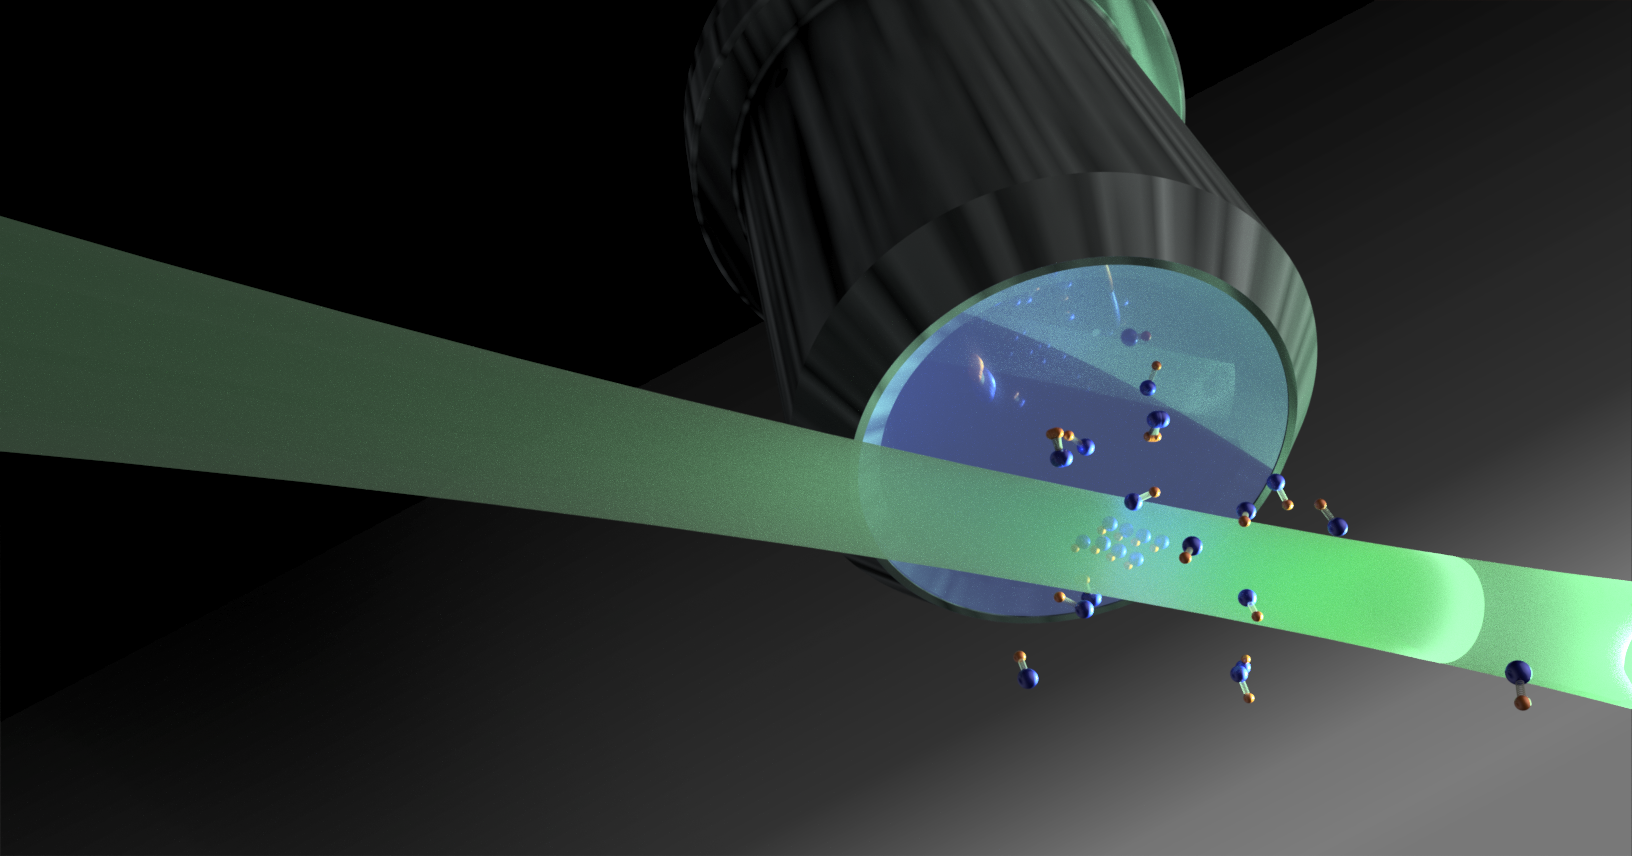
\includegraphics[width=\paperwidth]{front_bg.png}}
  }
  \setbeamercolor{title}{fg=cyan!50}
  \setbeamercolor{author}{fg=white}
  \setbeamercolor{institute}{fg=white}
  \setbeamercolor{date}{fg=white}
  \begin{frame}{}
    \titlepage
  \end{frame}
}

% Raman transfer
%% Next major goal of the experiment is to create a loosely
%% bound molecule in the optical tweezer to increase the wavefunction overlaps
%% with the ground state so that we can do the STIRAP.
%% We do this with Raman. Remember last time, tweezer scattering, 1038 tweezer.
\begin{frame}{}
  \begin{center}
    \begin{tikzpicture}
      \begin{scope}[scale=0.7]
        \draw[->,line width=1.2] (0, 0) -- (0, 8);
        \node[above,rotate=90] at (0, 4) {Energy};
        \draw[->,line width=1.2] (0, 0) -- (8, 0);
        \node[below] at (4, -0.5) {Internuclear distance};

        \draw[cyan!85!blue] (1.0269 + 0.25, 2.5) -- (7.25, 2.5);
        \draw[cyan!85!blue] (1.0793 + 0.25, -0.4631 + 2.5) -- (4.5 + 0.25, -0.4631 + 2.5);

        \draw[line width=1.1,cyan!85!blue]
        plot[samples=200,domain=1:7,variable=\x]
        ({\x + 0.25}, {6.8*\x^(-3.4)-6.5*\x^(-1.7) + 2.5});
        \node[cyan!85!blue] at (3.75, 1.0) {$a^3\Sigma^+$};

        \draw[line width=1.1,red]
        plot[samples=200,domain=1:7.5,variable=\x]
        ({\x - 0.75}, {9.2*\x^(-2.5)-9.0*\x^(-1.3) + 7.5});
        \node[above right,red] at (0.55, 7.2) {$c^3\Sigma^+$};

        \mytweezer.drawNaAtom(6.55, 2.6, 0.12)
        \mytweezer.drawCsAtom(7.05, 2.6, 0.10)

        \mytweezer.drawNaAtom(4.08, 2.15, 0.12)
        \mytweezer.drawCsAtom(4.25, 2.15, 0.10)

        \draw[black!40,dashed,line width=1] (0.25, 5) -- (7.25, 5);

        \draw[->,green!80!black,line width=0.8] (6.8, 2.7) -- (5.5, 5)
        node[midway, right, align=left] {$\approx1038\mathrm{nm}$\\\ \ \ Tweezer};
        \draw[->,green!80!black,line width=0.8] (5.45, 5) -- (4.165, 2.25);
      \end{scope}
      \visible<2->{
        \node[below right,align=center] at (6.5, 4.5) {No Rabi oscillation\\
          \\\\
          
\includegraphics[width=2.5cm]{crying_face.png}};
      }
    \end{tikzpicture}
  \end{center}
\end{frame}

% Not seeing oscillation

%% Verify states, both initial and final (motional states)
\begin{frame}{What can go wrong?}
  \begin{columns}
    \column{5cm}
    \begin{block}{State}
      \begin{itemize}
      \item<2-> Initial state (temperature)
      \item<3-> Final state
      \end{itemize}
    \end{block}
    \column{7cm}
    \vspace{-0.7cm}
    \begin{center}
      \visible<2->{\includegraphics[width=6cm]{init_temp.png}}
      \visible<3->{
        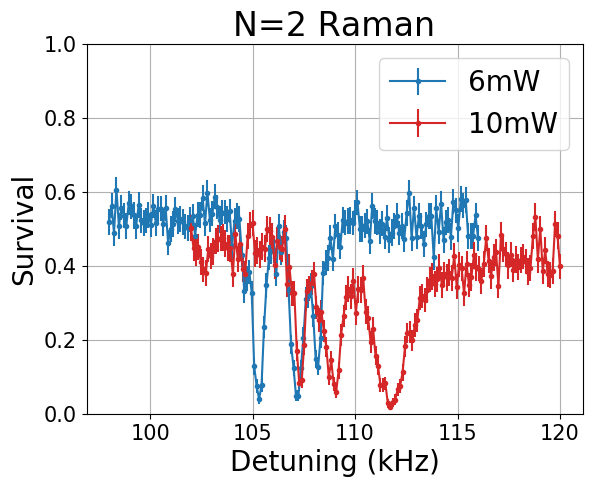
\includegraphics[width=5cm]{../../experiments/nacs_201810/imgs/data_20181103_raman_n2_6_10.png}
      }
    \end{center}
  \end{columns}
\end{frame}

%% Verify numbers by measuring different ....
%% delta, Omega_1, Omega_2, Gamma_1, Gamma_2 (Gamma, Delta)
\begin{frame}{}
  \begin{center}
    \begin{tikzpicture}
      \draw[line width=1] (-2, 0) -- (0, 0);
      \draw[line width=1] (-5, -2) -- (-3, -2);
      \visible<2->{
        \visible<-4>{
          \draw[->,line width=1,green!80!black]
          (-1, 0) -- (-4, -1.8) node[midway, right=0.4] {$\Omega_R$};
        }
        \draw[dashed,line width=0.7] (-5, -1.8) -- (-3, -1.8);
        \visible<-5>{
          \node[left] at (-5.1, -1.9) {$\delta$};
          \draw[->,line width=0.7] (-4.8, -1.4) -- (-4.8, -1.8);
          \draw[->,line width=0.7] (-4.8, -2.4) -- (-4.8, -2.0);
        }
      }
      \visible<3-5>{
        \draw[snakearrow,line width=1,red!80!black]
        (-0.8, 0) -- (0, 1.5) node[midway, left=0.1] {$\Gamma_1$};
        \draw[snakearrow,line width=1,orange!80!black]
        (-4.2, -2) -- (-5, -0.5) node[midway, right=0.1] {$\Gamma_2$};
      }
      \visible<4->{
        \node[right,align=left,red!80!black] at (1, 2) {$\Gamma_1$: PA rate};
        \node[right,align=left,orange!80!black] at (1, 1) {$\Gamma_2$: Line width};
        \node[right,align=left,green!80!black] at (1, 0) {$\Omega_R$: Transfer/decay rate};
        \node[right,align=left] at (1, -1) {$\delta$: Resonance/line width};
      }
      \visible<5->{
        \draw[line width=1] (-3.5, 4) -- (-1.5, 4);
        \draw[dashed,line width=0.7] (-3.5, 3.5) -- (-1.5, 3.5);
        \draw[->,line width=1,green!80!black] (-1, 0) -- (-2.45, 3.5)
        node[midway,right=0.1] {\only<6->{$\Omega_1$}};
        \draw[->,line width=1,green!80!black] (-2.55, 3.5) -- (-4, -1.8)
        node[midway,left=0.1] {\only<6->{$\Omega_2$}};
        \draw[<->,line width=0.7] (-3.3, 3.5) -- (-3.3, 4);
        \node[left] at (-3.6, 3.75) {$\Delta$};
      }
      \visible<6->{
        \draw[snakearrow,line width=1,blue!80!black] (-2, 4) -- (-1, 2.5)
        node[midway,right=0.1] {$\Gamma_e$};
        \node[below] at (0, -2.5) {$\Delta \rightarrow \Gamma_e\ \Omega_1\ \Omega_2$};
      }
    \end{tikzpicture}
  \end{center}
\end{frame}

% Possible issues
% * Fluctuation (light shift)
%%% Technical issue
%%% Measure without fluctuation effect
\begin{frame}{Detuning fluctuation}
  \begin{columns}
    \column{6cm}
    \begin{itemize}
    \item<+-> Raman Rabi rate $\Omega_R\propto\dfrac{\Omega_1\Omega_2}{\Delta}$\\
    \item<+-> Light shift $\delta_L\propto\dfrac{\Omega_1^2+\Omega_2^2}{\Delta}$\\
    \item<+-> For $\Omega_2\gg\Omega_1$\\\vspace{0.4cm}
      $\dfrac{\delta_L}{\Omega_R}\approx\dfrac{\Omega_2}{\Omega_1}\gg1$\\
    \item<+-> Raman linewidth\\\vspace{0.4cm}
      $\Gamma_2\propto\dfrac{1}{\Delta^2}$ or $\dfrac{\delta_L}{\Gamma_2}\propto\Delta$
    \end{itemize}
    \column{6cm}
    \begin{tikzpicture}
      \draw[line width=1] (-2, 0) -- (0, 0);
      \draw[line width=1] (-5, -2) -- (-3, -2);
      \draw[->,dashed,line width=1,green!80!black]
      (-1, 0) -- (-4, -1.8) node[midway, right=0.4] {$\Omega_R$};
      \draw[dashed,line width=0.7] (-5, -1.8) -- (-3, -1.8);
      \node[left] at (-5.1, -1.9) {$\delta$};
      \draw[->,line width=0.7] (-4.8, -1.4) -- (-4.8, -1.8);
      \draw[->,line width=0.7] (-4.8, -2.4) -- (-4.8, -2.0);
      \draw[snakearrow,line width=1,red!80!black]
      (-0.8, 0) -- (0, 1.5) node[midway, left=0.1] {$\Gamma_1$};
      \draw[snakearrow,line width=1,orange!80!black]
      (-4.2, -2) -- (-5, -0.5) node[midway, right=0.1] {$\Gamma_2$};
      \draw[line width=1] (-3.5, 4) -- (-1.5, 4);
      \draw[dashed,line width=0.7] (-3.5, 3.5) -- (-1.5, 3.5);
      \draw[->,line width=1,green!80!black] (-1, 0) -- (-2.45, 3.5)
      node[midway,right=0.1] {$\Omega_1$};
      \draw[->,line width=1,green!80!black] (-2.55, 3.5) -- (-4, -1.8)
      node[midway,left=0.1] {$\Omega_2$};
      \draw[<->,line width=0.7] (-3.3, 3.5) -- (-3.3, 4);
      \node[left] at (-3.6, 3.75) {$\Delta$};
      \draw[snakearrow,line width=1,blue!80!black] (-2, 4) -- (-1, 2.5)
      node[midway,right=0.1] {$\Gamma_e$};
    \end{tikzpicture}
  \end{columns}
\end{frame}

% * Coherence / Scattering ratio
%%% Larger linewidth (everything are roughly consistent except the larger linewidth)
%%% Verify directly
\begin{frame}{}
  \begin{columns}
    \column{6cm}
    \begin{itemize}
    \item<+-> Rabi frequencies ($\Omega_R$, $\Omega_1$, $\Omega_2$)\\
      and light shift ($\delta_L$) matches theory.
    \item<+-> Scattering is faster than expected.
    \item<+-> $\Gamma_e\approx2\pi\cdot300\mathrm{MHz}$
    \end{itemize}
    \column{6cm}
    \begin{center}
      \visible<+->{
        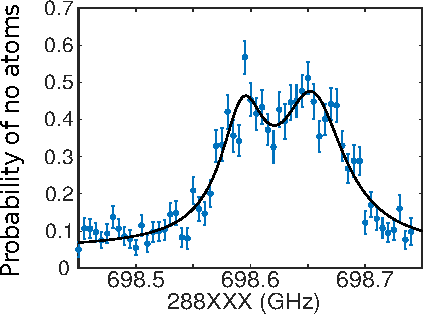
\includegraphics[width=5cm]{../damop-2018-poster/pa-v0}
      }
      \visible<+->{
        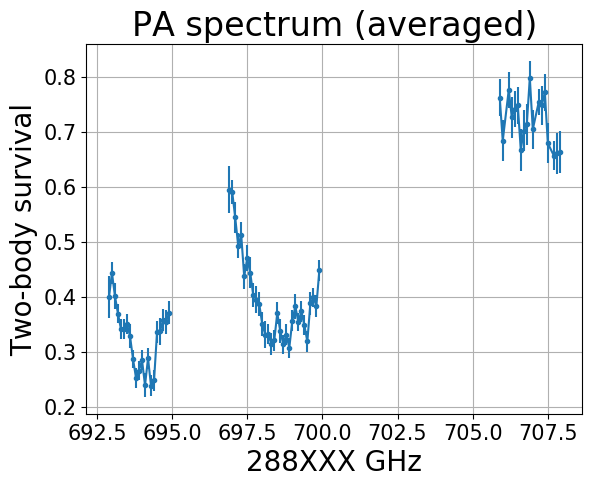
\includegraphics[width=5cm]{../../experiments/pa_201904/imgs/data_20190409_pa_avg}
      }
    \end{center}
  \end{columns}
\end{frame}

% What's next.
% * Beam size?
% * 2-Photon process
% * Different light, different excited states
\begin{frame}{Next}
  \begin{columns}
    \column{6cm}
    \begin{block}{Cause}
      \begin{itemize}
      \item<+-> PA beam size?
      \item<+-> Two photon process?
      \end{itemize}
    \end{block}
    \visible<3->{
      \begin{block}{Alternative}
        \begin{itemize}
        \item<+-> Different wavelength (976nm?)
        \item<+-> Different transfer path (singlet?)
        \end{itemize}
      \end{block}
    }
    \column{6cm}
    \begin{tikzpicture}
      \visible<2>{
        \draw[line width=1] (-2, 0) -- (0, 0);
        \draw[line width=1] (-5, -2) -- (-3, -2);
        \draw[dashed,line width=0.7] (-5, -1.8) -- (-3, -1.8);
        \draw[line width=1] (-3.5, 3) -- (-1.5, 3);
        \draw[dashed,line width=0.7] (-3.5, 2.5) -- (-1.5, 2.5);
        \draw[->,line width=1,green!80!black] (-1, 0) -- (-2.45, 2.5);
        \draw[->,line width=1,green!80!black] (-2.55, 2.5) -- (-4, -1.8);
        \draw[->,line width=2,green!80!black] (-2.5, 2.5) -- (-3, 5) node[right] {\textbf{???}};
      }
    \end{tikzpicture}
  \end{columns}
\end{frame}

\end{document}
